%%%%%%%%%%%%%%%%%%%%%%%%%%%%%%%%%%%%%%%%%%%%%%%%%
%
%     Chapter 4
%
%%%%%%%%%%%%%%%%%%%%%%%%%%%%%%%%%%%%%%%%%%%%%%%%

\chapter{Vector of $i2^k$}
\label{four}

Parabix operation works on full range of vector types. For 128-bit SIMD register, Parabix supports $v128i1$, $v64i2$, $v32i4$, \ldots, $v1i128$, we call them as the vector of $i2^k$. Vector types $vXi8$, $vXi16$, \ldots, $vXi64$ are widely used for multimedia processing, digital signal processing and Parabix technology. They are well supported by the LLVM infrastructure, but the remaining vector type with smaller elements are not well-supported. For instance, $vXi1$ is a natural view of many processor operations, like AND, OR, XOR; they are bitwise operations. However, $v32i1$, $v64i1$ and $v128i1$ are all illegal on current LLVM 3.4 back end for X86 architecture. After seeing a $v128i1$ vector, the type legalization phase promotes element type $i1$ to $i8$, and then split the vector to fit 128 bits register size; thus the incoming $v128i1$ turns into 8 $v16i8$ vectors. For bitwise-and on 2 $v128i1$ vectors, LLVM produces 8 pairs of AND on $v16i8$ together with operations to truncate and concatenate back the $v128i1$ result; while we can simply bitcast $v128i1$ to any legal 128-bit vector like $v4i32$, perform the bitwise-and and bitcast the result back to $v128i1$. The performance penalty of type legalization is high in this example. Another type legalization example of $v32i1$ can be found in Figure~\ref{figure:v32i1_legalize_type}.

\begin{figure}[ht!]
  \centering
  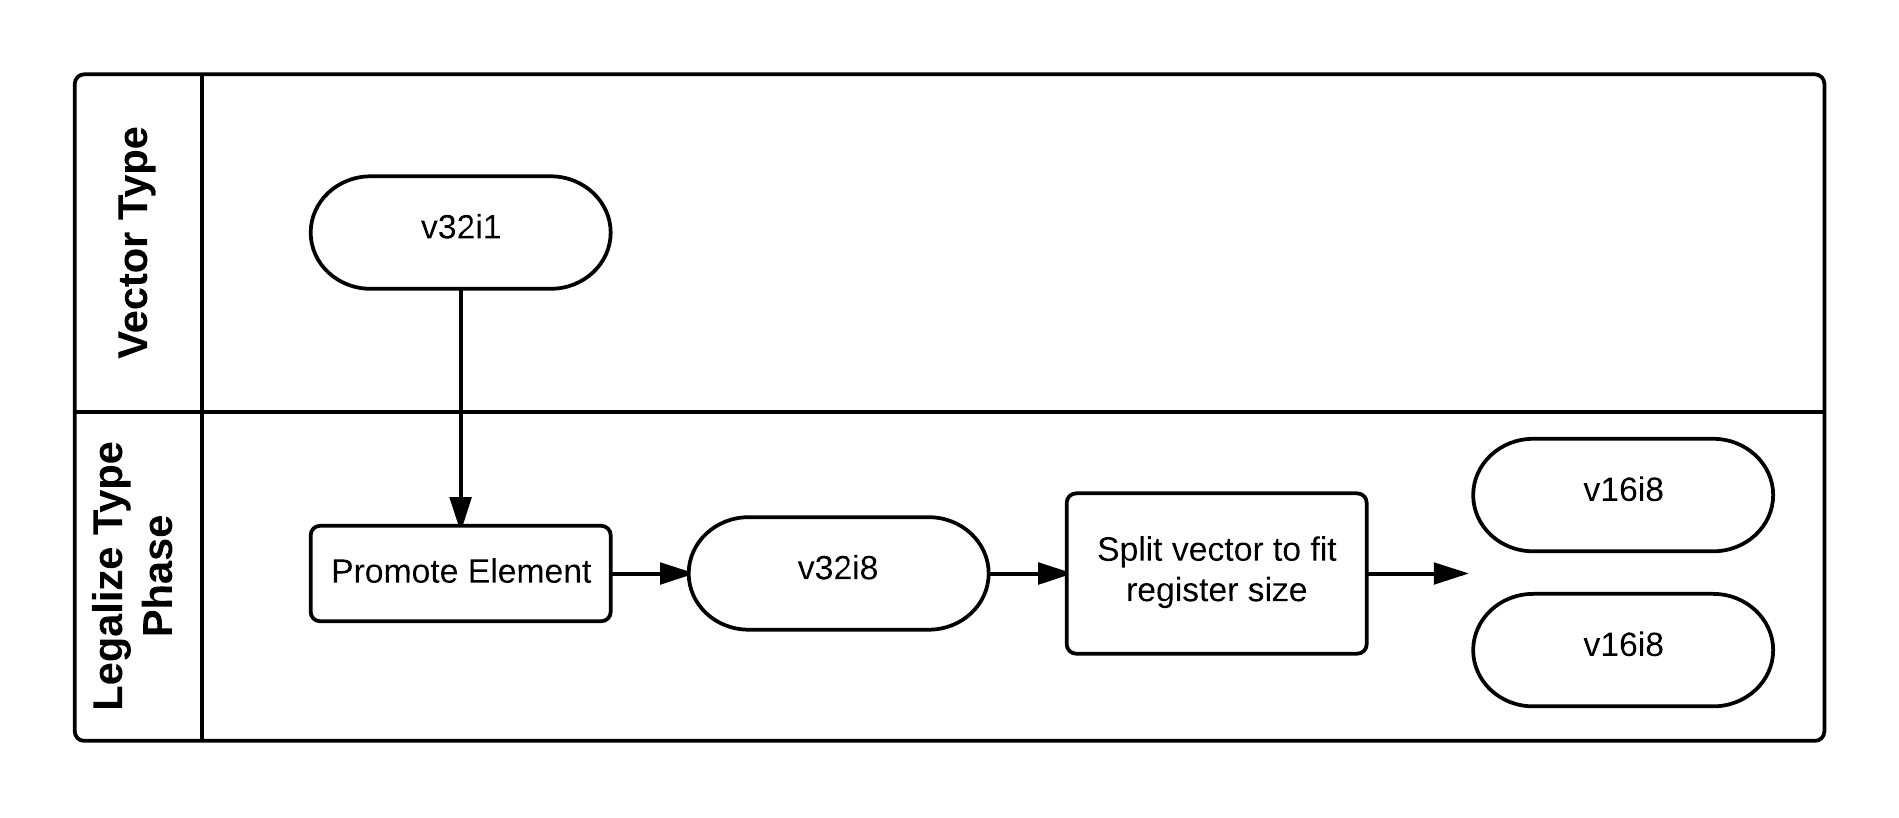
\includegraphics[width=140mm]{draw/v32i1_legalize_type.png}
  \caption{Type legalize process for $v32i1$ vector}
  \label{figure:v32i1_legalize_type}
\end{figure}

LLVM applies the same promote element strategy to vectors of $i2$ and $i4$, which leads to huge SelectionDAG generation and thus poor machine code. On the other hand, $i1$, $i2$ and $i4$ vectors are important to Parabix performance-critical operations, such as transposition and deletion; Parabix applications, such as DNA sequence (ATCG pairs) matching which can be encoded into $i2$ vectors most efficiently, requires a better support of small element vectors. The inductive doubling instruction set architecture (IDISA) which is the ideal model for Parabix needs a core set of functions on the $i2^k$ vectors as the first key element. All these reasons motivate us to find better implementation of $i1$, $i2$ and $i4$ vectors.

\section{Redefine Legality}

From Chapter~\ref{two} we know that LLVM has three ways to legalize vector types: Scalarization, Vector Widening and Vector Element Promotion. None of these strategies could legalize small element vectors properly. Think about $v32i1$: it fits in the general 32-bit registers, and we can not benefit from extending or splitting the vector in wider or more registers, not to mention scalarizing it. It is the best to store $v32i1$ vectors just in the general 32-bit register and properly handle the operations on them.

So we want to redefine the type legality inside LLVM\@. Instead of having direct hardware intrinsic on it, we define a vector type which has the same size in bits with one of the target's registers to be a legal vector type. The definition of the illegal operation remains the same. Under this definition, $v32i1$ is legal on any 32-bit platform, $v64i1$ is legal on any 64-bit platform and $v64i2$ is legal on any platform with 128-bit SIMD registers.

However, as more types are legal, we need to handle more illegal operations that are not directly supported by the processor. We implement every IR instruction that works on vectors except: (1) floating point instructions, because Parabix use integer operations exclusively. (2) division and remainder, because no Parabix operation require it. (3) shufflevector for vectors of small elements, because a general high-performance implementation of them are hard and unnecessary; instead we optimize some special cases that are used in the Parabix operations. To sum up, we implement the following instructions for the $i2^k$ vectors: (1) common binary functions listed in Table~\ref{table:semantics}; (2) basic vector operations like INSERT VECTOR ELT, EXTRACT VECTOR ELT and BUILD VECTOR\@.

LLVM has the facility to "expand" an illegal operation, so that some operations we did not implement are still available. For example $v32i1$, we did not lower its shufflevector but we can still write shufflevector on $v32i1$ in IR\@. LLVM could expand it into a sequence of extracting and inserting vector elements. Of course the performance is not good at all. Efficient shufflevector support is possible with the new instructions PEXT and PDEP introduced in the Intel Haswell BMI2. According to \cite{lee2001efficient}, arbitrary $n$-bit permutation can be done using no more than $\lg n$ GRP instructions. It means for arbitrary $v32i1$ shufflevector, no more than 10 PEXTs, 5 ORs and 5 SHIFTs are needed.

\section{In-place Lowering Strategy}

With the redefined legality, we provide the fourth way to legalize vector type: In-place Lowering. It is called "in-place" because we do not rearrange the bit value of the vector data, we look at the same data with a different type. A trivial example is the logical operations on \verb|<32 x i1>|; we can simply bitcast \verb|<32 x i1>| to $i32$ and perform the same operation. Almost all the operations on $vXi1$ can be simulated with a few logic operations on $iX$ (except the basic insert \& extract vector operations) as listed in Table~\ref{table:vxi1}. Figure~\ref{figure:v32i1_compare} shows the overall process of lowering $v32i1$ addition.

In-place Lowering allows us to copy the vector between registers or shift the vector within the register boundary. But it is different from vector element promotion. Refer to the Figure~\ref{figure:v8i4_v8i8}, vector element promotion requires shifting different element with different offsets.

\begin{figure}[ht!]
  \centering
  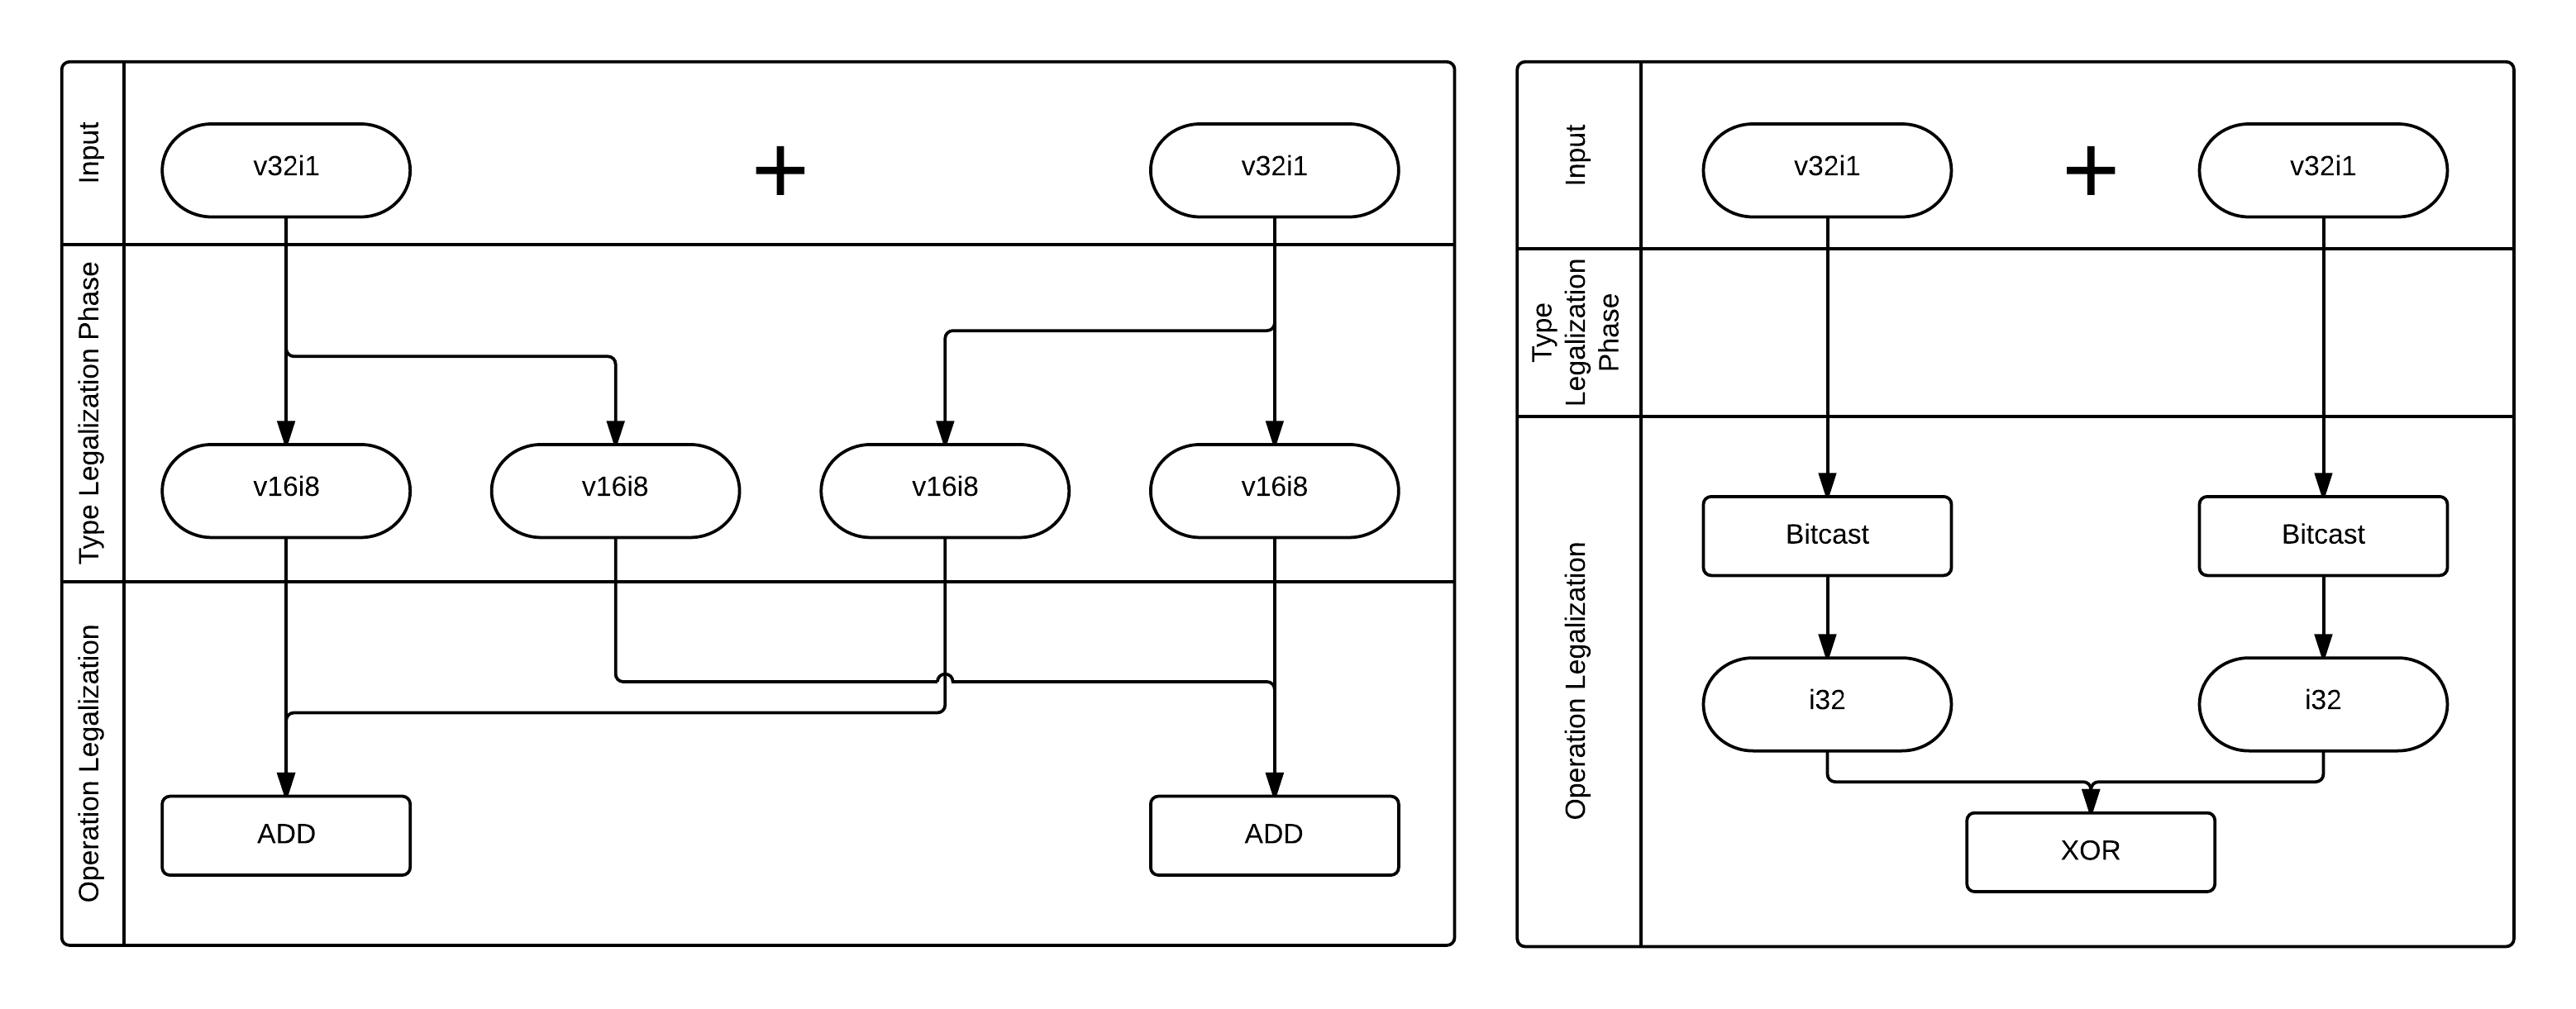
\includegraphics[width=150mm]{draw/v32i1_compare.png}
  \caption[Comparison between LLVM default legalize process and in-place lowering.]{Comparison between LLVM default legalize process (left) and in-place lowering (right). The right marks $v32i1$ type legal and handles the operation ADD in the operation legalization phase. This keeps the data in the general registers without being promoted or expanded.}
  \label{figure:v32i1_compare}
\end{figure}

\begin{table}
  \begin{center}
    \begin{tabular}{|l|l|}
      \hline
      Operation & Semantics \\ \hline
      ADD & $c_i = a_i + b_i$ \\\hline
      SUB & $c_i = a_i - b_i$ \\\hline
      MUL & $c_i = a_i * b_i$ \\\hline
      AND, OR, XOR & Common logic operations. \\\hline
      NE        & Integer comparison between vectors. $c_i = 1$ if $a_i$ is not equal to $b_i$.    \\ \hline
      EQ        & $c_i = 1$ if $a_i$ is equal to $b_i$                                  \\ \hline
      LT        & $c_i = 1$ if $a_i < b_i$. $a_i$ and $b_i$ is viewed as signed integer \\ \hline
      GT        & $c_i = 1$ if $a_i > b_i$. $a_i$ and $b_i$ is viewed as signed integer \\ \hline
      ULT       & Same with LT, but numbers are viewed as unsigned integer              \\ \hline
      UGT       & Same with GT, but numbers are viewed as unsigned integer              \\ \hline
      SHL       & $c_i = a_i << b_i$. Element wise shift left                            \\ \hline
      SRL       & $c_i = a_i >> b_i$. Element wise logic shift right                     \\ \hline
      SRA       & $c_i = a_i >> b_i$. Element wise arithmetic shift right                \\ \hline
    \end{tabular}
  \end{center}
  \caption[Supported operations and its semantics.]{Supported operations and its semantics. $A, B$ is the operands, $C$ is the result. $a_i, b_i, c_i$ is the $i_{th}$ element.}
  \label{table:semantics}
\end{table}

\begin{table}
  \begin{center}
    \begin{tabular}{|c|c|}
      \hline
      Operation on $vXi1$ & $iX$ equivalence \\ \hline
      ADD(A, B) & XOR(A', B') \\ \hline
      SUB(A, B) & XOR(A', B') \\ \hline
      MUL(A, B) & AND(A', B') \\ \hline
      AND(A, B) & AND(A', B') \\ \hline
      OR(A, B) & OR(A', B') \\ \hline
      XOR(A, B) & XOR(A', B') \\ \hline
      NE(A, B) & XOR(A', B') \\ \hline
      EQ(A, B) & NOT(XOR(A', B')) \\\hline
      LT(A, B), UGT(A, B) & AND(A', NOT(B')) \\\hline
      GT(A, B), ULT(A, B) & AND(B', NOT(A')) \\\hline
      SHL(A, B), SRL(A, B) & AND(A', NOT(B')) \\\hline
      SRA(A, B) & A' \\\hline
    \end{tabular}
  \end{center}
\caption[Legalize operations on $vXi1$ with $iX$ equivalence.]{Legalize operations on $vXi1$ with $iX$ equivalence. A, B are $vXi1$ vectors, A', B' are $iX$ bitcasted from $vXi1$. For $v128i1$, we use $v2i64$ instead of $i128$ since LLVM supports the former better.}
\label{table:vxi1}
\end{table}

\subsection{Lowering for $vXi2$}
Vector type $vXi2$ has important role in the IDISA model and Parabix transposition and inverse transposition. Ideal Three-Stage Parallel Transposition\cite{transposition} requires \verb|hsimd<4>::packh| and \verb|hsimd<4>::packl|, which can be implemented with shufflevectors on $v64i2$. Shufflevectors of $v64i2$ are also required by Ideal Inverse Transposition, for \verb|esimd<2>::mergeh| and \verb|esimd<2>::mergel|. Transposition is the first step of every parabix application\cite{inductive_doubling_principle}. It is also a significant overhead for some application like regular expression matching\cite{rob_regex}. So good code generation for $vXi2$ is important.

Lowering $vXi2$ is harder than $vXi1$, so we propose a systematic framework using logic and 1-bit shifting operations. Consider $A, B$ as two $i2$ integers, $A=a_0a_1$ and $B=b_0b_1$, we can construct a truth table for every operation $C = OP(A, B)$. We then calculate the first bit and the second bit of $C$ separately with the logic combinations of $a_0, a_1, b_0, b_1$ and turn this into \textit{Circuit Minimization Problem}: find minimized Boolean functions for $c_0$ and $c_1$. We use Quine-McCluskey algorithm\cite{johnson1981quine} to solve it; an example can be found in Table~\ref{table:quine}.

\begin{table}[h]
  \centering
  \begin{tabular}{ccc}
    \hline
    A                   & B                   & C                  \\ \hline
    00                  & 00                  & 00                 \\
    00                  & 01                  & 01                 \\
    00                  & 10                  & 10                 \\
    \multicolumn{3}{c}{$\ldots$}                                        \\
    11                  & 11                  & 10                 \\ \hline
  \end{tabular}

  \begin{tabular}{lll}
    \\
    \multicolumn{3}{c}{$c_0 = (a_0 \oplus b_0) \oplus (a_1 \land b_1)$} \\
    \multicolumn{3}{c}{$c_1 = a_1 \oplus b_1$}
  \end{tabular}
  \caption{Truth-table of ADD on 2-bit integers and the minimized Boolean functions for $C$.}
  \label{table:quine}
\end{table}

Once we get the minimized Boolean functions, we can apply it onto the whole $vXi2$ vector. To do this, we need {\tt IFH1(Mask, A, B)} which selects bits from vector {\tt A} and {\tt B} according to the {\tt Mask}. If the $i_{th}$ bit of {\tt Mask} is $1$, $\text{\tt A}_i$ is selected, otherwise $\text{\tt B}_i$ is selected. {\tt IFH1(Mask, A, B)} simply equals to $(\text{\tt Mask} \land \text{\tt A}) \lor (\lnot \text{\tt Mask} \land \text{\tt B})$. With {\tt IFH1}, if we have calculated the all high bits ($c_0$ for all the element) and low bits ($c_1$ for all the element), we can combine them with special {\tt HiMask}, which equals to $101010 \ldots 10$, 128 bits long in binary. To calculate all the high bits of each $i2$ element, we bitcast A, B into full register type (e.g.\ $v32i1$ to $i32$, $v64i2$ to $i128$ or $v2i64$) and then do the following substitution on the minimized Boolean functions:

\begin{itemize}
    \item For $a_0$ and $b_0$, replace it with $A$ and $B$.
    \item For $a_1$ and $b_1$, replace it with $A << 1$ and $B << 1$.
    \item Keep all the logic operations.
\end{itemize}

So $c_0 = (a_0 \oplus b_0) \oplus (a_1 \land b_1)$ becomes $(A \oplus B) \oplus ((A << 1) \land (B << 1))$, which simplifies to $(A \oplus B) \oplus ((A \land B) << 1)$. We use shifting to move every $a_1$ and $b_1$ in place. For all the lower bits of each $i2$ element, the rules are similar:

\begin{itemize}
    \item For $a_1$ and $b_1$, replace it with $A$ and $B$.
    \item For $a_0$ and $b_0$, replace it with $A >> 1$ and $B >> 1$.
    \item Keep all the logic operations.
\end{itemize}

Program~\ref{program:genloweradd} is the actual custom code to lower $v64i2$ addition. One thing to mention here is that we deploy a template system to automatically generate custom lowering code and the corresponding testing code. We describe the template system later in Chapter~\ref{five}.

\begin{program}
\begin{verbatim}
static SDValue GENLowerADD(SDValue Op, SelectionDAG &DAG) {
  MVT VT = Op.getSimpleValueType();
  MVT FullVT = getFullRegisterType(VT);
  SDNodeTreeBuilder b(Op, &DAG);

  if (VT == MVT::v64i2) {
    SDValue A = b.BITCAST(Op.getOperand(0), FullVT);
    SDValue B = b.BITCAST(Op.getOperand(1), FullVT);

    return b.IFH1(/* 10101010...10, totally 128 bits */
                  b.HiMask(128, 2),
                  /* C0 = (A0 ^ B0) ^ (A1 & B1) */
                  b.XOR(b.XOR(A, B), b.SHL<1>(b.AND(A, B))),
                  /* C1 = (A1 ^ B1)*/
                  b.XOR(A, B));
  }

  llvm_unreachable("GENLower of add is misused.");
  return SDValue();
}
\end{verbatim}
\caption{The function generated to lower ADD on $v64i2$.}
\label{program:genloweradd}
\end{program}

\subsection{Inductive Doubling Principle For $i4$ Vector}
Now we have better code generation for $vXi1$ and $vXi2$, $vXi4$ vectors are our next optimization target. Shufflevectors of $vXi4$ are used in \verb|hsimd<8>::packh|, \verb|hsimd<8>::packl| and \verb|esimd<4>::mergeh|, which are required by Ideal Three-Stage Transposition / Inverse Transposition; $vXi4$ is also the critical part of the IDISA model. But unfortunately, the strategies discussed above cannot be applied to $vXi4$ efficiently.

Circuit Minimization Problem is NP-hard\cite{quine1952problem, kabanets2000circuit}. For $vXi4$, 4 Boolean functions of 8 variables are necessary: $c_i = f_i(a_0, a_1, a_2, a_3, b_0, b_1, b_2, b_3), i \in \left\{{0, 1, 2, 3}\right\}$. It is known that most Boolean functions on $n$ variables have circuit complexity at least $2^n/n$\cite{kabanets2000circuit} and we need 1-bit, 2-bit, 3-bit shifting on $A$, $B$. So the framework on $vXi2$ could not generate efficient code for us at this time. Instead, we introduce \textit{Inductive Doubling Principle} \cite{inductive_doubling_principle} and we show that this general principle can be applied for $vXi4$ and even wider vector element type, e.g.\ multiplication on $v16i8$, to get better performance.

\begin{figure}[ht!]
\centering
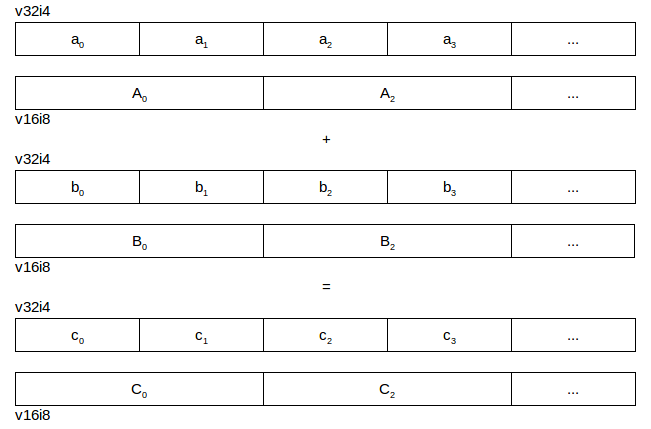
\includegraphics[width=110mm]{draw/add_4.png}
\caption[Addition of two $v32i4$ vectors.]{To add 2 $v32i4$ vectors, $a$ and $b$, we bitcast them into $v16i8$ vectors. The lower 4 bits of $A_0 + B_0$ gives us $c_1$. We then mask out $a_1$ and $b_1$ (set them to zero), do add again, and the higher 4 bits of the sum is $c_0$.}
\label{figure:add_4}
\end{figure}

\begin{figure}[ht!]
\centering
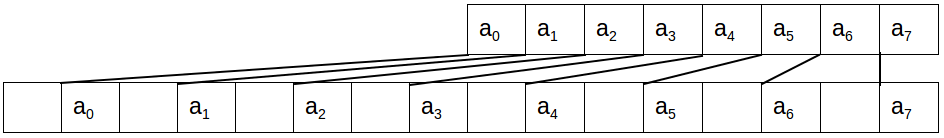
\includegraphics[width=130mm]{draw/v8i4_v8i8.png}
\caption[LLVM default type legalization of $v8i4$ to $v8i8$.]{LLVM default type legalization of $v8i4$ to $v8i8$. $a_0$ to $a_7$ are $i4$ elements and they are shifted with different offsets during the element type promotion.}
\label{figure:v8i4_v8i8}
\end{figure}

We use $v32i4$ as an example to illustrate Inductive Doubling Principle. To legalize $v32i4$, LLVM promotes this type into $v32i8$, widen every element to $i8$ then shift every element except the first one. Figure~\ref{figure:v8i4_v8i8} shows an example of widening $v8i4$ into $v8i8$, we can see unnecessary movement of vector element during widening. On a platform with 128 bits SIMD register, $v32i8$ is further divided into two $v16i8$ and requires 2 registers to hold, while the original type $v32i4$ has 128 bits in size and should be able to reside in only 1 register. Inductive Doubling Principle could achieve the latter for us. It bitcasts the vector in-place, view the same register as $v16i8$ type and emulate $i4$ operations with $i8$; e.g.\ in Figure~\ref{figure:add_4}, to get \verb|add <32 x i4> %a, %b|, we calculate $c_0, c_2, \ldots, c_{30}$ (high 4 bits in each $i8$ element) and $c_1, c_3, \ldots, c_{31}$ (low 4 bits in each $i8$ element) separately with 2 $v16i8$ additions:

\begin{gather}
C = \text{\tt IFH1}(HiMask_8, A \land HiMask_8 + B \land HiMask_8, A + B) \\
HiMask_8 = (1111000011110000 \ldots 11110000)_2
\end{gather}

So we can emulate SIMD operations on $iX$ vectors with $iX/2$ or $i2X$ vector operations. We implemented all the operations on $vXi4$ with this principle and the algorithm is listed in Table~\ref{table:vXi4}. One thing needs to explain is SETCC, which is the internal representation of integer comparison in LLVM\@. It has a third operand to determine comparison type, such as SETEQ (equal), SETLT (signed less than), and SETUGE (unsigned greater or equal to). The third operand preserves in our algorithm.

\begin{table}[h]
\centering
\begin{tabular}{ccc}
\multicolumn{3}{c}{$C = \text{\tt IFH1}(HiMask_8, HiBits, LowBits)$} \\ \hline
\multicolumn{1}{|c|}{\multirow{2}{*}{\begin{tabular}[c]{@{}c@{}}Operation\\ $v32i4$\end{tabular}}} & \multicolumn{1}{c|}{$HiBits$} & \multicolumn{1}{c|}{$LowBits$} \\ \cline{2-3}
\multicolumn{1}{|c|}{} & \multicolumn{2}{c|}{All operation is on $v16i8$} \\ \hline
\multicolumn{1}{|c|}{MUL} & \multicolumn{1}{c|}{$MUL(A >> 4, B >>4) << 4$} & \multicolumn{1}{c|}{Default} \\ \hline
\multicolumn{1}{|c|}{SHL} & \multicolumn{1}{c|}{$SHL(A \land HiMask_8, B >>4)$} & \multicolumn{1}{c|}{$SHL(A, B \land LowMask_8)$} \\ \hline
\multicolumn{1}{|c|}{SRL} & \multicolumn{1}{c|}{$SRL(A, B>>4)$} & \multicolumn{1}{c|}{$SRL(A \land LowMask_8, B \land LowMask_8)$} \\ \hline
\multicolumn{1}{|c|}{SRA} & \multicolumn{1}{c|}{$SRA(A, B>>4)$} & \multicolumn{1}{c|}{$SRA(A << 4, (B \land LowMask_8)) >> 4$} \\ \hline
\multicolumn{1}{|c|}{SETCC} & \multicolumn{1}{c|}{Default} & \multicolumn{1}{c|}{$SETCC(A << 4, B << 4)$} \\ \hline
\multicolumn{1}{|c|}{Default OP} & \multicolumn{1}{c|}{$OP(A \land HiMask_8, B \land HiMask_8)$} & \multicolumn{1}{c|}{$OP(A, B)$} \\ \hline
\multicolumn{1}{l}{In the table:} & \multicolumn{1}{l}{} & \multicolumn{1}{l}{} \\
 & \multicolumn{2}{l}{$A >> 4$: logic shift right every $i8$ element by 4 bits} \\
 & \multicolumn{2}{l}{$A << 4$: shift left of every $i8$ element by 4 bits} \\
\multicolumn{1}{l}{} & \multicolumn{2}{l}{$HiMask_8 = (11110000 \ldots 11110000)_2$} \\
\multicolumn{1}{l}{} & \multicolumn{2}{l}{$LowMask_8 = (00001111 \ldots 00001111)_2$}
\end{tabular}
\caption[Algorithm to lower $v32i4$ operations.]{Algorithm to lower $v32i4$ operations. The legalization input is $c = OP(a, b)$, where $a, b, c$ are $v32i4$ vectors. $A, B, C$ is the bitcasted results from $a, b, c$. They are all $v16i8$ type.}
\label{table:vXi4}
\end{table}

Furthermore, this method is applicable to vectors of wider element type. Multiplication on $v16i8$, for example, generates poor code on LLVM 3.4 (Program~\ref{program:mult_8}): the vectors are finally scalarized and 16 multiplications on $i8$ elements are generated. With in-place promotion, we bitcast the operands into $v8i16$ and generate 2 SIMD multiplications ($pmullw$) instead.

\begin{program}
\begin{verbatim}
define <16 x i8> @mult_8(<16 x i8> %a, <16 x i8> %b) {
entry:
  %c = mul <16 x i8> %a, %b
  ret <16 x i8> %c
}
\end{verbatim}
\rule{\textwidth}{1pt}

\begin{multicols}{2}
\begin{verbatim}
# LLVM 3.4 default:
  pextrb▸ $1, %xmm0, %eax
  pextrb▸ $1, %xmm1, %ecx

  mulb▸   %cl
  movzbl▸ %al, %ecx
  pextrb▸ $0, %xmm0, %eax
  pextrb▸ $0, %xmm1, %edx

  mulb▸   %dl
  movzbl▸ %al, %eax
  movd▸   %eax, %xmm2
  pinsrb▸ $1, %ecx, %xmm2
  pextrb▸ $2, %xmm0, %eax
  pextrb▸ $2, %xmm1, %ecx

  mulb▸   %cl
  movzbl▸ %al, %eax
  pinsrb▸ $2, %eax, %xmm2
  pextrb▸ $3, %xmm0, %eax
  pextrb▸ $3, %xmm1, %ecx

  mulb▸   %cl
  movzbl▸ %al, %eax
  pinsrb▸ $3, %eax, %xmm2
  pextrb▸ $4, %xmm0, %eax
  pextrb▸ $4, %xmm1, %ecx
  ...
  ...
  (16 mulb blocks in total)

            (a)
\end{verbatim}
\columnbreak
\begin{verbatim}
# Inductive doubling result:
  movdqa▸ %xmm0, %xmm2
  pmullw▸ %xmm1, %xmm2
  movdqa▸ .LCPI0_0(%rip), %xmm3
  movdqa▸ %xmm3, %xmm4
  pandn▸  %xmm2, %xmm4
  psrlw▸  $8, %xmm1
  psrlw▸  $8, %xmm0
  pmullw▸ %xmm1, %xmm0
  psllw▸  $8, %xmm0
  pand▸   %xmm3, %xmm0
  por▸    %xmm4, %xmm0
  retq

            (b)
\end{verbatim}
\end{multicols}
\caption[Comparison of the compiled machine code of $v16i8$ multiplication between LLVM 3.4 and inductive doubling principle.]{LLVM 3.4 generate poor machine code for $v16i8$ multiplication. (a) is the generated code from LLVM 3.4. It $pextrb$ every $i8$ field and multiply them with $mulb$. The overall process in (a) is sequential. (b) is the generated code from inductive doubling principle. In (b), two $pmullw$ which is the multiplication on $v8i16$ are used to improve performance.}
\label{program:mult_8}
\end{program}

However, the algorithm in Table~\ref{table:vXi4} cannot guarantee the best performance. Addition on $v32i4$ requires 2 $v16i8$ additions, but we can actually implement it with one. Look back to Figure~\ref{figure:add_4}, we need to mask out $a_1$, $b_1$ and do add again, because $a_1 + b_1$ may produce carry bit to the high 4 bits. If we mask out only the high bit of $a_1$ and $b_1$, still we do not produce carry and we can calculate $c_0$ and $c_1$ together in one $v16i8$ addition. All we need to solve is how to put the high bit back. The following equations describe the 1-add algorithm:

\begin{gather}
  m = (10001000 \ldots 1000)_2 \\
  A_h = m \land A \\
  B_h = m \land B \\
  z = (A \land \lnot A_h) + (B \land \lnot B_h) \label{eq:1_add_z}\\
  r = r \oplus A_h \oplus B_h \label{eq:1_add_r}
\end{gather}

Equation~\eqref{eq:1_add_z} uses only one $v16i8$ addition and equation~\eqref{eq:1_add_r} put the high bit back. Our vector legalization framework is flexible enough that we can choose to legalize $v32i4$ addition with 1-add algorithm while keeping the remaining $v32i4$ operations under general in-place promotion strategy. We discuss our framework implementation in Chapter~\ref{five}.

\section{LLVM Vector Operation of $i2^k$}
In addition to the binary operations listed in Table~\ref{table:semantics}, LLVM provides convenient vector operations like \textit{insertelement}, \textit{extractelement} and \textit{shufflevector}, internally, they are DAG node INSERT VECTOR ELT, EXTRACT VECTOR ELT and VECTOR SHUFFLE\@. Another important internal node is BUILD VECTOR\@. In this section, we discuss how to custom lower these nodes on $i2^k$ vectors.

BUILD VECTOR takes an array of scalars as input and returns a vector with these scalars as elements. Take $v64i2$ vector on X86 SSE2 architecture for an example; ideally, the input provides an array of 64 $i2$ scalars and they are then assembled into a $v64i2$ vector. More specifically, since $i2$ is illegal on all X86 architecture, the legal input is actually 64 $i8$ scalars. The naive approach is to create an "empty" $v64i2$ vector, truncate every $i8$ into $i2$ and insert them into the proper location of the "empty" vector. We propose a better approach by rearranging the index.

Let us denote the input array as $a_0, a_1, \ldots, a_{63}$, $a_i$ are all $i8$. We rearrange them according to Table~\ref{table:build_vector} and build 4 $v16i8$ vectors $V_1, V_2, V_3, V_4$. The final build result is:
\begin{equation}
  V = V_1 \lor (V_2 << 2) \lor (V_3 << 4) \lor (V_4 << 6)
\end{equation}

\begin{table}[h]
\centering
\begin{tabular}{|p{1cm}|p{1cm}|p{1cm}|p{1cm}|p{1cm}|p{1cm}|r}
\cline{1-6}
$a_{60}$ & $\ldots$ & $a_{12}$ & $a_8$ & $a_4$ & $a_0$ & $V_1$ \\ \cline{1-6}
$a_{61}$ & $\ldots$ & $a_{13}$ & $a_9$ & $a_5$ & $a_1$ & $V_2$ \\ \cline{1-6}
$a_{62}$ & $\ldots$ & $a_{14}$ & $a_{10}$ & $a_6$ & $a_2$ & $V_3$ \\ \cline{1-6}
$a_{63}$ & $\ldots$ & $a_{15}$ & $a_{11}$ & $a_7$ & $a_3$ & $V_4$ \\ \cline{1-6}
\end{tabular}
\caption{Rearranging index for BUILD VECTOR on $v64i2$}
\label{table:build_vector}
\end{table}

SIMD OR and SHL are used in this formula, thus improving the performance by parallel computing. Rearranging index approach can be easily generalized to fit BUILD VECTOR of $v128i1$ and $v32i4$.

EXTRACT VECTOR ELT takes 2 operands, a vector $V$ and an index $i$. It returns the $i_{th}$ element of $V$. The semantic does not allow much parallelism in the implementation. On X86 architecture, there are built-in intrinsic to extract vector element, such as $pextrb$ ($i8$), $pextrw$ ($i16$), $pextrd$ ($i32$) and $pextrq$ ($i64$); for smaller element type, we could extract the wider integer that contains it, shift the small element to the lowest bits and truncate. Following algorithm gives an example of extracting the $i_{th}$ element from the $v64i2$ vector {\tt V}.

\begin{itemize}
  \item Bitcast {\tt V} to $v4i32$ {\tt V'} and extract the proper $i32$ {\tt E}. Since every $i32$ contains 16 $i2$ elements, the index of {\tt E} is $\lfloor i / 16 \rfloor$.
  \[\text{\tt V'} = \text{\tt bitcast <64 x i2> V to <4 x i32>} \]
  \[\text{\tt E} = \text{\tt extract element V',} \lfloor i / 16 \rfloor \]
  \item Shift right {\tt E}, to put the element we want in the lowest bits.
  \[\text{\tt E'} = \text{\tt E >>} (2 \times (i \bmod 16))\]
  \item Truncate the high bits of {\tt E'} to get the result.
  \[\text{\tt R} = \text{\tt truncate i32 E' to i2}\]
\end{itemize}

The choice of $v4i32$ does not make a difference, we can use any of the wider element vector type mentioned above. On the X86 architecture, the support of extraction on $v8i16$ starts at SSE2, while others start at SSE4.1, so we choose $v8i16$ extraction in our code to target broader range of machines.

INSERT VECTOR ELT is similar, it takes 3 operands, a vector $V$, an index $i$ and an element $e$. It inserts $e$ into the $i_{th}$ element of $V$ and returns the new vector. Same as EXTRACT VECTOR ELT, X86 SSE2 supports $v8i16$ insertion ($pinsrw$), SSE4.1 supports $v16i8$ ($pinsrb$), $v4i32$ ($pinsrd$) and $v2i64$ ($pinsrq$); for smaller element type, we could extract the wider integer that contains the element, modify the integer and insert it back. Following algorithm gives an example of inserting {\tt e} into the $i_{th}$ element of the $v64i2$ vector {\tt V}.

\begin{itemize}
  \item Bitcast {\tt V} to $v4i32$ {\tt V'} and extract the proper $i32$ {\tt E}.
  \[\text{\tt V'} = \text{\tt bitcast <64 x i2> V to <4 x i32>} \]
  \[\text{\tt E} = \text{\tt extract element V',} \lfloor i / 16 \rfloor \]

  \item Truncate {\tt e} and shift it to the correct position.
  \[\text{\tt e'} = \text{\tt zero extend (e} \land (11)_2 \text{\tt ) to i32} \]
  \[\text{\tt f} = \text{\tt e' <<} (2 \times (i \bmod 16))\]

  \item Mask out old content in {\tt E}, put in the new element.
  \[\text{\tt m} = (11)_2 << (2 \times (i \bmod 16)) \]
  \[\text{\tt E'} = (\text{\tt E} \land \lnot \text{\tt m}) \lor \text{\tt f}\]

  \item Insert back {\tt E'} to generate the new vector {\tt R}.
  \[\text{\tt R} = \text{\tt insert element V', E',} \lfloor i / 16 \rfloor \]
\end{itemize}

We have discussed VECTOR SHUFFLE in Chapter~\ref{three}. We did not develop a general lowering strategy for the small element VECTOR SHUFFLE\@. Instead, we focused more on special cases that matter to Parabix critical operations, we optimized those cases to match performance of the hand-written library.

\section{Long Stream Addition}
Parabix technology has the concept of adding 2 unbounded streams and of course this needs to be translated into a block-at-a-time implementation\cite{rob_regex}. One important operation is unsigned addition of 2 SIMD registers with carry-in and carry-out bit e.g.\ \verb|add i128 %a, %b| or \verb|add i256 %a, %b| with $i1$ carry-in bit \verb:c_in: and generates $i1$ carry-out bit \verb:c_out:. Cameron et al\cite{rob_regex} developed a general model using SIMD methods for efficient long-stream addition up to 4096 bits.

In this section, we replace the internal logic of wide integer addition ($i128$, $i256$ etc. ) of LLVM with the Parabix long-stream addition. Following Cameron at el\cite{rob_regex}, we assume the following SIMD operations on $i64$ vectors legal on the target:
\begin{itemize}
    \item \verb|add <N x i64> X, Y|, where $\text{\tt N} = RegisterSize / 64$. SIMD addition on each corresponding element of the $i64$ vectors, no carry bits could cross the element boundary.
    \item \verb|icmp eq <N x i64> X, -1|: compare each element of {\tt X} with the all-one constant, returning an \verb|<N x i1>| result.
    \item \verb|signmask <N x i64> X|: collect all the sign bit of $i64$ elements into a compressed \verb|<N x i1>| vector. From the LLVM speculation, this operation is equivalent to \verb|icmp lt <N x i64> X, 0|, which is the signed less-than comparison of each $i64$ element with 0. In the real implementation we use target-specific operations for speed, e.g. $movmsk\_pd$ for SSE2 and $movmsk\_pd\_256$ for AVX.
    \item Normal bitwise logic operations on \verb|<N x i1>| vectors. For small {\tt N}, native support may not exist, so we bitcast \verb|<N x i1>| to $iN$ and then zero extend it to $i32$. This conversion could also help with the 1-bit shift we use later.
    \item \verb|zext <N x i1> m to <N x i64>|: this corresponds to \verb|simd<64>::spread(X)| in \cite{rob_regex}. The internal logic of LLVM zero extension for $vNi1$ is not good enough, so we implement our own. An example of $v2i1$ is in Table~\ref{table:spread_v2i1}.
\end{itemize}

\begin{table}[h]
\centering
\begin{tabular}{|c|r|}
\hline
\multicolumn{2}{|c|}{Spread 2-bit value $(\text{\tt ab})_2$ to $v2i64$} \\ \hline
$M_0$                                                       & \verb'ab'              \\ \hline
$M_1 = M_0 \times \text{\tt 0x8001}$                        & \verb'...............ab.............ab' \\ \hline
$M_2 = M_1 \land  \text{\tt 0x10001}$                       & \verb'...............a...............b' \\ \hline
$M_3 = $ \text{\tt bitcast} $M_2$ \text{\tt to} $v2i16$     & \verb'<2 x i16> <i16 a, i16 b>' \\ \hline
$M_4 = $ \text{\tt zext} $M_3$ \text{\tt to} $v2i64$        & \verb'<2 x i64> <i64 a, i64 b>' \\ \hline
\end{tabular}
\caption{Example of spreading $v2i1$ to $v2i64$}
\label{table:spread_v2i1}
\end{table}

We then present the long stream addition of 2 $N \times 64$ bit values {\tt X} and {\tt Y} with these operations as the following.
\begin{enumerate}
    \item Get the vector sums of {\tt X} and {\tt Y}.
    \[\text{\tt R} = \text{\tt add <N x i64> X, Y} \]
    \item Get sign masks of {\tt X}, {\tt Y} and {\tt R}.
    \[\text{\tt x} = \text{\tt signmask <N x i64> X} \]
    \[\text{\tt y} = \text{\tt signmask <N x i64> Y} \]
    \[\text{\tt r} = \text{\tt signmask <N x i64> R} \]
    \item Compute the carry mask {\tt c}, bubble mask {\tt b} and the increment mask {\tt i}.
    \[\text{\tt c} = (\text{\tt x} \wedge \text{\tt y}) \vee ((\text{\tt x} \vee \text{\tt y}) \wedge \neg \text{\tt r})\]
    \[\text{\tt b} = \text{\tt icmp eq <N x i64> R, -1}\]
    \[\text{\tt i} = \text{\tt MatchStar(c*2+c\_in, b)}\]
    MatchStar is a key Parabix operation which is developed for regular expression matching:
    \[\text{\tt MatchStar}(M, C) = (((M \wedge C) + C)  \oplus C) | M\]
    \item Compute the final result {\tt Z} and carry-out bit {\tt c\_out}.
    \[\text{\tt S} = \text{\tt zext <N x i1> i to <N x i64>}\]
    \[\text{\tt Z} = \text{\tt add <N x i64> R, S}\]
    \[\text{\tt c\_out} = \text{\tt i >> N}\]
    One note here for the mask type: {\tt c} and {\tt i} are literally all \verb|<N x i1>| vectors, but we actually bitcast and zero extend them into $i32$. This is useful in the formula {\tt c*2+c\_in}, {\tt MatchStart} and {\tt i >> N}; in fact, after we shift left {\tt c} by {\tt c*2}, we already have an $N+1$ bit integer which does not fit in \verb|<N x i1>| vector. The same is true for {\tt i}; so when we write {\tt zext <N x i1> i to <N x i64>}, there is an implicit truncating to get the lower {\tt N} bits of {\tt i}, but when we shift right {\tt i} by {\tt i >> N}, we do not do such truncation.
\end{enumerate}

LLVM internally implement long integer addition with a sequence of ADDC and ADDE, which is just chained 64-bit additions (or 32-bit additions on 32-bit target). We replace that with the long stream addition model thus improving the performance by parallel computing. As the hardware evolves, wider SIMD registers would be introduced, like 512-bit register in Intel AVX512, our general implementation could easily adopt this change in hardware and add two $i512$ in constant time.

During our implementation, we found there was no intrinsic in IR for addition with carry-in and carry-out bit, there was only one intrinsic {\tt uadd.with.overflow} for addition with carry-out bit. To realize unbounded stream addition, the ability to take carry-in bit is necessary, otherwise we would end up with two {\tt uadd.with.overflow} to include the carry-in bit. So we introduced a new intrinsic {\tt uadd.with.overflow.carryin} and backed it with the long stream addition algorithm.
